\chapter{TINJAUAN PUSTAKA}

% Ubah konten-konten berikut sesuai dengan isi dari tinjauan pustaka
\section{Hasil Penelitian Terdahulu}
Pada penelitian sebelumnya telah dilakukan dalam rangka menginvestigasi implementasi deteksi objek secara \textit{real time} berbasis \textit{YOLO (You Only Look Once)} \cite{redmon2016you}. Selain itu, terdapat juga penelitian yang memfokuskan pada pengembangan metode deteksi postur yoga menggunakan platform \textit{MediaPipe} \cite{garg2022yoga}. Penelitian selanjutnya telah membahas tentang penggunaan \textit{MediaPipe} dan \textit{Machine Learning} dalam mendeteksi posisi bagi keperluan pelatihan \cite{supanich2023machine}. Sebuah studi lainnya telah mengkaji penggunaan \textit{MediaPipe} dalam memonitor latihan bicep curl dengan tujuan penguatan otot \cite{nguyen2023assessing}. Selanjutnya, dalam konteks yang berbeda, terdapat penelitian yang melibatkan penggunaan model \textit{Faster-RCNN-Inception-V2-COCO} dari \textit{TensorFlow} dalam melakukan pengenalan gestur semaphore menggunakan bendera \cite{motty2023flag}. Metode ini memanfaatkan \textit{TensorFlow API} dan Model \textit{Deep Neural Network (DNN)} dalam melatih model dan melakukan deteksi gestur semaphore.

Pada penelitian-penelitian tersebut, pendekatan pasif digunakan dalam menganalisis dan mengidentifikasi objek, postur yoga, posisi pelatihan, serta gestur semaphore. Melalui penggunaan teknologi yang canggih, seperti \textit{YOLO}, \textit{MediaPipe}, \textit{Machine Learning}, dan model \textit{Deep Neural Network (DNN)}, para peneliti telah mampu mencapai deteksi yang efisien dan akurat. Penelitian-penelitian ini berkontribusi dalam memperluas pemahaman dan penerapan teknologi dalam berbagai bidang, mulai dari deteksi objek hingga pengenalan gestur semaphore dengan bantuan komputasi yang kuat.

\section{Bendera Semaphore}
\begin{figure}[hbt!]
  \centering
	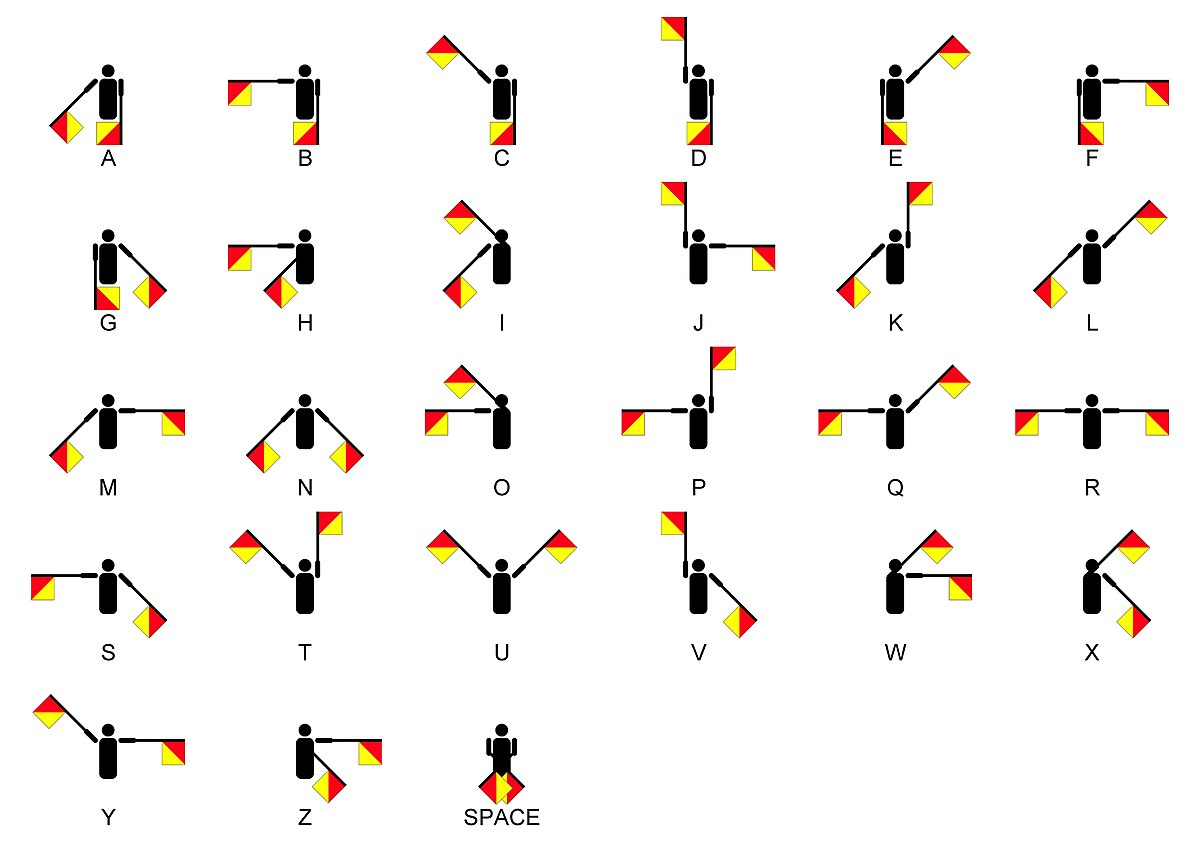
\includegraphics[width=0.7\linewidth]{gambar/bener/Semaphore-Pose.jpg}
	\captionof{figure}{Bendera Semaphore \cite{wiki_semafor_bendera} }
	\label{fig:BenderaSemaphore}
\end{figure}

Bendera Semaphore adalah sebuah sistem komunikasi yang dikembangkan pada abad ke-18 oleh Claude Chappe, seorang ahli matematika Prancis, sebagai cara mengirim pesan telegraf tanpa menggunakan kabel \cite{8752707}. Dalam sistem ini, dua bendera yang dapat digerakkan ke posisi yang berbeda digunakan dalam mewakili huruf dan angka dalam alfabet seperti \ref{fig:BenderaSemaphore}. Melalui pengaturan posisi bendera-bendera tersebut, pesan dapat ditransmisikan kepada penerima pesan tanpa memerlukan infrastruktur kabel yang rumit. Bendera Semaphore umumnya digunakan dalam situasi di mana komunikasi jarak jauh diperlukan, seperti antara kapal atau kota-kota yang terpisah \cite{gundogdu2019semaphore}.

Penggunaan sistem komunikasi bendera Semaphore membawa manfaat yang signifikan pada masa ketika teknologi komunikasi belum mencapai tingkat kemajuan seperti sekarang. Pesan dapat dikirim dengan cepat dan efisien tanpa ketergantungan pada koneksi kabel yang terbatas pada waktu itu. Dalam era tersebut, peran sistem ini dalam meningkatkan efektivitas dan kecepatan pertukaran informasi antarlokasi yang terpisah tidak dapat diabaikan. Komunikasi jarak jauh menjadi lebih efisien dan andal berkat sistem bendera Semaphore yang ditemukan oleh Claude Chappe pada abad ke-18. Dengan demikian, dapat disimpulkan bahwa bendera Semaphore merupakan sebuah sistem komunikasi yang menggunakan dua bendera yang dapat diposisikan ke berbagai posisi agar bisa mengirimkan pesan jarak jauh. Sistem ini ditemukan oleh Claude Chappe pada abad ke-18 sebagai solusi mengatasi keterbatasan koneksi kabel pada masa itu. Pemanfaatan bendera Semaphore membawa manfaat yang signifikan dalam meningkatkan efisiensi dan keandalan komunikasi jarak jauh pada era tersebut.

\section{Estimasi Pose}
Estimasi pose adalah suatu teknik atau metode yang sangat relevan dan berharga dalam berbagai bidang aplikasi, seperti augmented reality, robotika, pemrosesan citra, dan pengenalan gerakan. Kemampuan memperkirakan dengan tepat posisi dan orientasi objek dalam ruang tiga dimensi memungkinkan pengembangan solusi yang lebih canggih dan tepat dalam berbagai konteks.Dalam konteks penggunaan kamera, estimasi pose menjadi semakin penting karena berbagai kemajuan dalam teknologi kamera dan sensor, termasuk sensor kamera dengan resolusi tinggi, kamera multi-view, dan bahkan kamera yang terintegrasi dengan sensor kedalaman. Keberadaan data sensor yang kaya memberikan potensi besar  meningkatkan akurasi dan ketepatan estimasi pose.

Proses estimasi pose bisa menjadi tantangan tersendiri karena melibatkan beberapa langkah kompleks. Pertama-tama, data sensor yang relevan harus dikumpulkan dengan hati-hati, dan hal ini dapat melibatkan pengaturan kamera yang tepat, kalibrasi, dan penyesuaian parameter sensor lainnya. Selanjutnya, langkah kritis berikutnya adalah mengidentifikasi fitur-fitur penting dalam data sensor yang didapatkan, seperti menemukan titik-titik referensi, tepi, atau fitur-fitur geometris lainnya. Pemilihan fitur yang tepat dan akurat adalah kunci utama kesuksesan dalam estimasi pose. Setelah fitur-fitur relevan diidentifikasi, langkah selanjutnya adalah mencocokkan atau membandingkan fitur-fitur tersebut dengan fitur-fitur yang diketahui atau telah direkam sebelumnya. Metode pencocokan ini dapat sangat bervariasi, dan tergantung pada jenis data sensor yang digunakan dan konteks aplikasi. Dalam beberapa kasus, estimasi pose juga melibatkan pencocokan dengan model geometris atau model 3D objek yang diketahui, yang memerlukan komputasi yang lebih rumit dan penggunaan algoritma yang lebih canggih.  \cite{Andriluka_2014_CVPR}

Di era modern ini, terutama dengan perkembangan pesat dalam bidang kecerdasan buatan, teknik estimasi pose semakin dipengaruhi oleh pendekatan berbasis \textit{Deep Learning}. Penggunaan jaringan saraf tiruan dan model \textit{deep neural network} telah membuktikan kehebatannya dalam memahami fitur-fitur kompleks dalam data sensor dan menghasilkan estimasi pose yang lebih akurat dan dapat diandalkan. Namun, kendati perkembangan teknologi yang pesat, tantangan dalam estimasi pose masih ada, terutama ketika menghadapi situasi yang kompleks dan tidak terstruktur. Selain itu, faktor lingkungan seperti pencahayaan, bayangan, dan perubahan kondisi sekitar juga dapat mempengaruhi kualitas estimasi pose. Oleh karena itu, para peneliti terus bekerja meningkatkan teknik estimasi pose dengan menggabungkan pendekatan-pendekatan yang berbeda, mengoptimalkan algoritma yang ada, dan menggunakan data sensor yang semakin canggih.

Dalam beberapa tahun terakhir, metode estimasi pose telah menjadi fokus utama dalam penelitian dan pengembangan di berbagai industri. Penggunaan augmented reality dalam permainan dan aplikasi lainnya semakin menuntut akurasi estimasi pose yang lebih tinggi. Di bidang robotika, kemampuan robot mengenali dan memahami posisi objek di sekitarnya sangat penting bagi keberhasilan tugas yang rumit dan kompleks. Bahkan dalam pemrosesan citra dan pengenalan gerakan, estimasi pose berperan penting dalam analisis dan pengolahan data. \cite{Toshev_2014_CVPR} . Secara keseluruhan, estimasi pose adalah bidang yang menarik dan penting, dengan aplikasi yang meluas dan beragam. Dengan terus majunya teknologi sensor dan perkembangan dalam bidang kecerdasan buatan, diharapkan estimasi pose akan terus berkembang dan memberikan kontribusi yang signifikan dalam berbagai industri dan aplikasi kehidupan sehari-hari.

\section{MediaPipe}
\textit{MediaPipe} merupakan sebuah \textit{framework} yang sangat fleksibel dan efisien dalam mengelola dan memproses input sensori seperti video dan audio. Dikembangkan oleh tim \textit{Google Research}, \textit{MediaPipe} menyediakan beragam komponen persepsi yang dapat digabungkan dengan mudah dalam membuat prototipe dan mengembangkan aplikasi canggih yang dapat dijalankan di berbagai platform. Keunggulan \textit{MediaPipe} terletak pada kemampuannya mengoptimalkan penggunaan sumber daya dengan mengurangi latensi, menangani sinkronisasi data seri waktu, serta melakukan pengukuran kinerja dan konsumsi sumber daya. Dengan performa yang baik dan efisiensi dalam pemrosesan input sensori, \textit{MediaPipe} menjadi pilihan yang menarik bagi para pengembang aplikasi. Salah satu komponen unggulan dalam \textit{MediaPipe} adalah Estimasi Posisi Manusia (\textit{Human Pose Estimation}). Estimasi Pose Manusia merupakan teknik yang bertujuan mendeteksi dan mengidentifikasi posisi tubuh manusia dalam gambar atau video. Dengan menggunakan algoritma dan model yang ada dalam \textit{MediaPipe}, pengembang dapat dengan mudah mengintegrasikan kemampuan ini ke dalam aplikasi mereka. Estimasi Pose Manusia memungkinkan analisis lanjutan terhadap posisi tubuh manusia dalam video atau gambar, membuka peluang mengembangkan berbagai aplikasi yang melibatkan interaksi manusia. \cite{lugaresi2019mediapipe}
\begin{figure}[hbt!]
  \centering
  % Nama dari file gambar yang diinputkan
  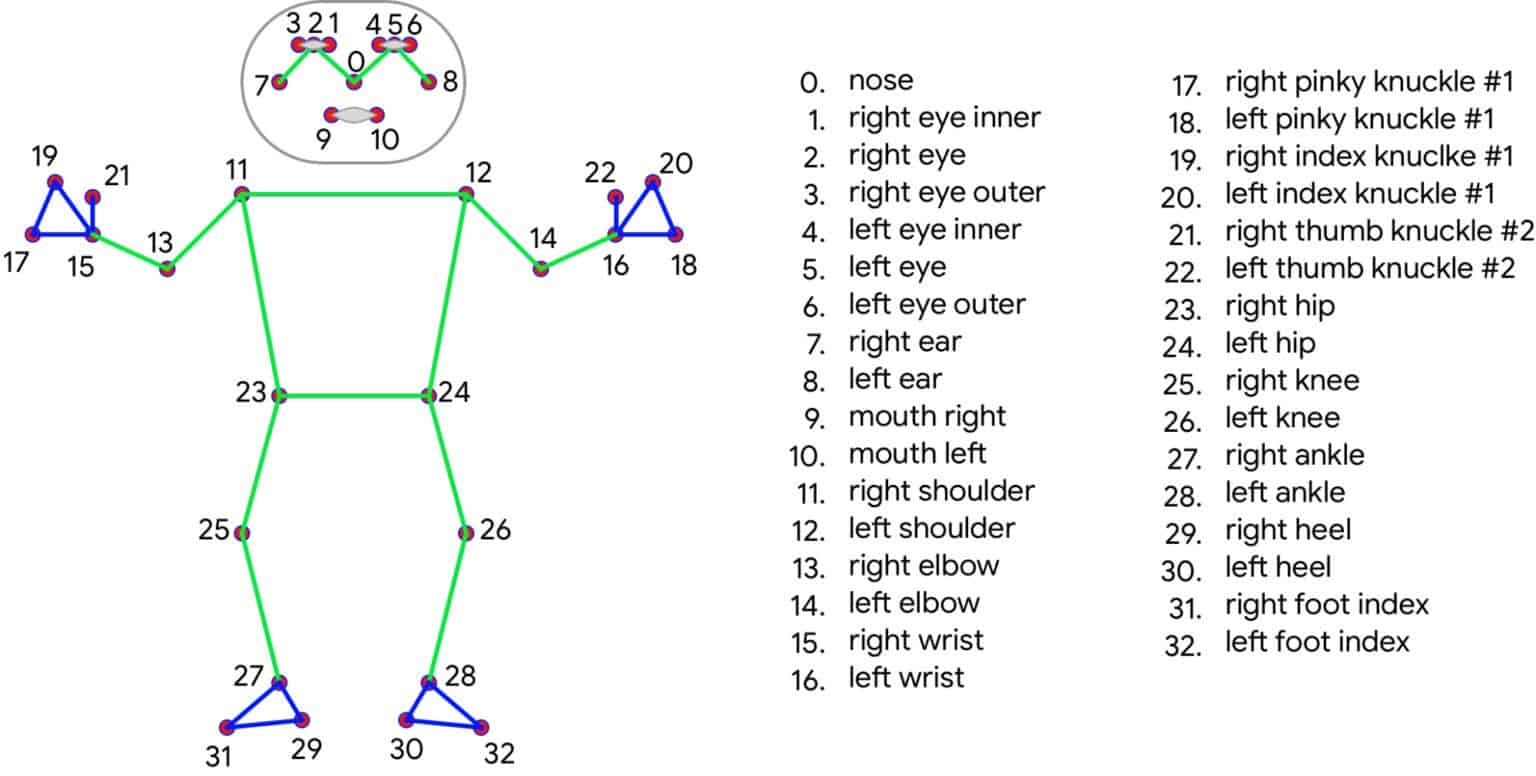
\includegraphics[width=0.7\linewidth]{gambar/humanpose.jpg} 
  % Keterangan gambar yang diinputkan
  \captionof{figure}{Human Pose Skeleton MediaPipe \cite{google_mediapipe}}
  % Label referensi dari gambar yang diinputkan
  \label{fig:Pose Tubuh dari MediaPipe}
\end{figure}
Sebagai contoh, dengan memanfaatkan Estimasi Pose Manusia dari \textit{MediaPipe} seperti pada Gambar \ref{fig:Pose Tubuh dari MediaPipe} , pengembang dapat menciptakan aplikasi deteksi gerakan yang mengenali gerakan tubuh pengguna saat mengendalikan perangkat atau berinteraksi dengan aplikasi secara intuitif. Aplikasi semacam ini sangat relevan dalam industri game dan realitas virtual, di mana interaksi alami dan lancar dengan dunia virtual menjadi sangat diinginkan. Selain itu, Estimasi Pose Manusia juga memungkinkan pengenalan gestur tubuh, di mana aplikasi dapat mengenali dan menafsirkan gerakan tangan atau tubuh pengguna sebagai perintah atau kontrol khusus. Contohnya adalah dalam pengembangan aplikasi \textit{sign language recognition} yang dapat menerjemahkan gerakan bahasa isyarat menjadi teks atau ucapan, membantu komunikasi bagi orang-orang dengan gangguan pendengaran. \cite{singh2021real}

Fitur Estimasi Pose Manusia juga dapat dimanfaatkan dalam bidang olahraga dan rehabilitasi fisik. Dalam olahraga, aplikasi dapat mengukur dan menganalisis postur tubuh atlet memberikan umpan balik dan perbaikan teknik. Sedangkan dalam rehabilitasi fisik, aplikasi dapat membantu pasien mengikuti latihan fisioterapi dengan benar dengan mengenali postur tubuh mereka dan memberikan petunjuk visual atau suara.Dalam lingkungan penelitian, Estimasi Pose Manusia dapat digunakan dalam analisis gerakan manusia, seperti dalam studi biomekanika, pengenalan tindakan manusia, atau pengamatan perilaku manusia. Data posisi tubuh manusia yang akurat dan real-time yang diberikan oleh \textit{MediaPipe} mempermudah peneliti melakukan analisis yang mendalam terhadap berbagai aspek gerakan manusia. Salah satu konsep yang mendukung kemampuan Estimasi Pose Manusia dalam \textit{MediaPipe} adalah \textit{Human Pose Skeleton} (\textit{kerangka tubuh manusia}). \textit{MediaPipe} menghasilkan representasi kerangka tubuh manusia dalam bentuk \textit{skeleton} yang terdiri dari serangkaian titik-titik kunci (\textit{keypoints}) yang menggambarkan posisi sendi-sendi dan bagian tubuh manusia. Informasi tentang posisi sendi-sendi ini memberikan gambaran yang sangat berguna tentang postur dan gerakan tubuh manusia dalam video atau gambar. 

Titik-titik \textit{landmark} tersebut terdiri dari berbagai bagian tubuh, seperti kepala, leher, bahu, siku, pergelangan tangan, panggul, lutut, hingga pergelangan kaki. Total jumlah \textit{landmark} yang digunakan dalam Mediapipe adalah 33 titik. Setiap titik \textit{landmark} ini memiliki koordinat yang menunjukkan posisi relatif terhadap citra atau frame video yang sedang dianalisis. Dengan informasi titik-titik \textit{landmark} ini, Mediapipe dapat mengkonstruksi pose skeleton dengan menghubungkan titik-titik tersebut sesuai dengan struktur anatomi tubuh manusia. Hasil dari pendeteksian pose skeleton ini dapat digunakan dalam berbagai tujuan, seperti analisis gerakan tubuh, klasifikasi aktivitas manusia, pembuatan animasi, dan pengenalan gerakan.

\textit{MediaPipe} menyediakan \textit{skeleton} dengan akurasi tinggi dan kemampuan pelacakan yang andal. Selain itu, \textit{skeleton} tersebut dapat diintegrasikan dengan mudah ke dalam aplikasi lain atau digunakan sebagai input berbagai tugas analisis dan pengenalan gerakan. Representasi \textit{skeleton} ini memberikan representasi yang ringkas namun informatif tentang tubuh manusia, sehingga memudahkan pengembang dan peneliti bekerja dengan data pose manusia.Secara keseluruhan, Fitur Estimasi Pose Manusia yang berasal dari \textit{Human Pose Skeleton} , Fitur \textit{MediaPipe} adalah fitur yang kuat dan berguna dalam mengolah input sensori berupa video dan gambar. Dengan kemampuan ini, \textit{MediaPipe} membuka peluang yang luas bagi pengembangan aplikasi interaktif, analisis gerakan, pengenalan gestur, hingga aplikasi di bidang olahraga dan rehabilitasi fisik. Kecepatan dan efisiensi \textit{MediaPipe} dalam mengelola sumber daya membuatnya menjadi pilihan utama bagi pengembang yang ingin menciptakan aplikasi canggih dan berdaya saing tinggi.

\section{Deep Learning}
\begin{figure}[hbt!]
  \centering
	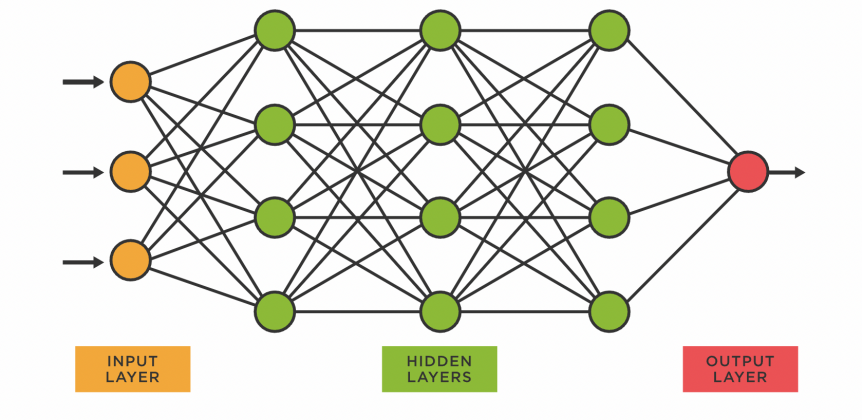
\includegraphics[width=0.9\linewidth]{gambar/bener/ArsitekturDeeplearning.png}
	\captionof{figure}{Deep Learning Layers \cite{tibco_neural_network}}
	\label{fig:Deep Learning secara umum}
\end{figure}  
\textit{Deep learning} adalah salah satu cabang utama dalam bidang kecerdasan buatan yang bertujuan mengembangkan model komputasional berdasarkan arsitektur jaringan saraf tiruan atau yang biasa disebut sebagai \textit{neural networks} yang sangat dalam dan kompleks seperti pada Gambar \ref{fig:Deep Learning secara umum}. Tujuan utama dari \textit{deep learning} adalah menciptakan mesin-mesin yang dapat belajar secara mandiri melalui representasi data yang lebih abstrak dan terstruktur. Para peneliti dan ilmuwan dalam bidang ini berupaya meniru cara kerja otak manusia, khususnya dalam hal pemrosesan informasi dalam lapisan-lapisan yang semakin kompleks dan hierarkis. \textit{Deep Learning} bekerja dengan mengimplementasikan jaringan saraf tiruan yang terdiri dari banyak lapisan atau tingkatan, yang masing-masing lapisan berisi sejumlah neuron. Setiap neuron menerima input, mengalikan input dengan bobot yang ditentukan, menjumlahkan hasil perkalian, dan lalu melewatkan hasilnya melalui fungsi aktivasi yang menghasilkan output. Proses ini berulang melalui lapisan-lapisan hingga mencapai lapisan keluaran, di mana output akhir model diperoleh. \textit{Deep learning} berusaha meniru cara kerja otak manusia dengan memproses data secara hierarkis dan mempelajari representasi fitur dari data yang kompleks. \cite{patterson2017deep}

Pada awal pelatihan, bobot dan bias pada setiap neuron diinisialisasi secara acak. Kemudian, model diberi data latihan yang terdiri dari input dan output yang diharapkan. Selama pelatihan, model mengoptimalkan bobot dan biasnya dapat meminimalkan kesalahan antara output yang dihasilkan oleh model dan output yang diharapkan. Proses ini dilakukan menggunakan algoritma optimasi seperti \textit{Stochastic Gradient Descent (SGD)} atau varian lainnya. Proses pelatihan \textit{deep learning} melibatkan dua tahap utama: tahap maju \textit{(forward pass)} dan tahap mundur \textit{(backward pass)}. Pada tahap maju, input diteruskan melalui model dari lapisan masukan ke lapisan keluaran, menghasilkan prediksi model. Selama tahap mundur, kesalahan prediksi dibandingkan dengan output yang diharapkan, dan nilai gradien kesalahan dihitung mundur melalui jaringan. Gradien ini menunjukkan bagaimana bobot dan bias pada setiap neuron harus diubah agar kesalahan dapat diminimalkan. \cite{deng2014deep}

Dengan adanya gradien kesalahan, algoritma optimasi dapat diterapkan dalam memperbarui bobot dan bias pada setiap neuron. Proses ini disebut pembaruan parameter. Algoritma optimasi menggunakan gradien ini menyesuaikan bobot dan bias agar model semakin mendekati target yang diinginkan. Pelatihan \textit{deep learning} memerlukan banyak data dan komputasi yang kuat. Model \textit{deep learning} memiliki banyak parameter, dan agar mendapatkan hasil yang baik, perlu data pelatihan yang mencukupi agar model dapat menggeneralisasi dengan baik pada data baru. Selain itu, model \textit{deep learning} juga membutuhkan sumber daya komputasi yang besar, seperti GPU atau TPU, dalam rangka mengatasi kompleksitas perhitungan pada model yang dalam dan besar. Setelah model dilatih, ia dapat digunakan melakukan tugas-tugas tertentu seperti klasifikasi gambar, analisis teks, atau prediksi. Model \textit{deep learning} juga dapat disimpan dan digunakan kembali melakukan tugas-tugas serupa atau dimodifikasi dan disesuaikan dengan tugas yang berbeda. Sebagai subbidang dalam machine learning, \textit{deep learning} terus mengalami perkembangan pesat. Para peneliti terus mencari cara-cara agar meningkatkan efisiensi, akurasi, dan generalisasi model \textit{deep learning}. \cite{smith2007teaching}

Salah satu turunan dari \textit{deep learning} adalah \textit{convolutional neural networks (CNN)}. \textit{CNN} terbukti sangat efektif dalam menangani masalah pengenalan gambar karena menggunakan operasi konvolusi dalam mendeteksi fitur-fitur khusus di dalam gambar. Sebagai contoh, ketika melakukan klasifikasi gambar mobil, \textit{CNN} mampu belajar mengenali roda, pintu, dan bagian-bagian mobil lainnya yang relevan dalam mengidentifikasi jenis mobil tersebut. Turunan lainnya adalah \textit{recurrent neural networks (RNN)}, yang khusus digunakan sebagai data urutan atau sequential seperti teks dan suara. \textit{RNN} mempertahankan informasi sebelumnya dalam bentuk "memori" dan digunakan pada tugas-tugas seperti prediksi teks berikutnya dalam suatu kalimat atau bahkan menerjemahkan bahasa.

Salah satu contoh lain turunan dari \textit{deep learning} adalah \textit{Generative Adversarial Networks (GANs)}. \textit{GANs} adalah suatu jenis model \textit{deep learning} yang terdiri dari dua jaringan saraf tiruan yang saling bersaing: generator dan diskriminator. Generator bertugas membuat data baru yang menyerupai data pelatihan, sementara diskriminator bertugas membedakan data asli dari data yang dihasilkan oleh generator. Proses pelatihan \textit{GANs} berlangsung dalam dua tahap yang berulang: generator mencoba meningkatkan kualitas data yang dihasilkan agar dapat menipu diskriminator, sedangkan diskriminator terus belajar menjadi lebih baik dalam membedakan data asli dan palsu.

Contoh lainnya adalah \textit{Autoencoders}, yang merupakan jenis jaringan saraf tiruan yang diajarkan merekonstruksi data masukan sebagai outputnya sendiri. \textit{Autoencoders} terdiri dari dua bagian: encoder yang mengonversi data masukan menjadi representasi terkompresi dalam ruang fitur yang lebih rendah, dan decoder yang mengubah representasi terkompresi kembali ke dalam bentuk data semula. \textit{Autoencoders} sering digunakan dalam tugas-tugas seperti reduksi dimensi data (dimensionality reduction) dan denoising, di mana model ini belajar merepresentasikan data dalam bentuk yang lebih efisien dan tangguh terhadap noise. Turunan \textit{deep learning} lainnya adalah \textit{Long Short-Term Memory (LSTM)}, yang merupakan varian dari \textit{recurrent neural networks (RNN)} yang lebih mampu dalam mengatasi masalah vanishing gradient pada data urutan panjang. \textit{LSTM} memiliki mekanisme "gerbang" khusus yang memungkinkannya menyimpan informasi dalam waktu yang lebih lama dan mengatur aliran informasi pada lapisan tersembunyi. Akibatnya, \textit{LSTM} menjadi populer dalam aplikasi NLP seperti penerjemahan mesin, pembangkitan teks, dan analisis sentimen.

\textit{Deep learning} telah berhasil diimplementasikan dalam berbagai bidang dan memberikan dampak yang signifikan. Salah satu contoh implementasi \textit{deep learning} yang menonjol adalah di bidang pengenalan gambar dan pengolahan citra. Model \textit{deep learning} seperti \textit{Convolutional Neural Networks (CNN)} telah digunakan melakukan klasifikasi gambar, deteksi objek, dan segmentasi citra. Misalnya, aplikasi pengenalan wajah di perangkat lunak atau perangkat keamanan yang dapat mengidentifikasi individu berdasarkan fitur wajahnya. Dalam bidang kesehatan, \textit{deep learning} telah digunakan mendukung diagnosis medis dan penelitian. Model \textit{deep learning} telah diterapkan dalam mendeteksi penyakit dari gambar medis seperti \textit{X-ray},\textit{ CT scan}, atau MRI. Selain itu, \textit{deep learning} juga digunakan dalam analisis citra histopatologi membantu mendiagnosis kanker dan penyakit lainnya. Penerapan \textit{deep learning} juga dapat ditemukan di bidang otomotif, khususnya dalam pengembangan kendaraan otonom. Model \textit{deep learning} seperti \textit{CNN} dan \textit{LSTM} digunakan mengenali objek di sekitar kendaraan, memprediksi perilaku pengendara, dan membantu dalam mengambil keputusan saat berkendara.

Dalam industri keuangan, \textit{deep learning} telah digunakan dalam analisis data keuangan dan prediksi pasar. Model \textit{deep learning} dapat mengidentifikasi pola kompleks dari data pasar dan membantu investor atau trader dalam membuat keputusan investasi. Penerapan \textit{deep learning} juga ditemukan dalam aplikasi \textit{NLP (Natural Language Processing)}. Model \textit{deep learning} seperti \textit{Transformer} telah digunakan dalam penerjemahan bahasa, generasi teks, analisis sentimen, dan \textit{chatbot}. Selain itu, \textit{deep learning} juga telah diadopsi dalam berbagai aplikasi industri seperti manufaktur, pertanian, energi, dan lainnya. Misalnya, dalam industri manufaktur, \textit{deep learning} digunakan dalam mengoptimalkan proses produksi dan memprediksi kerusakan pada mesin. Di bidang pertanian, \textit{deep learning} digunakan mendeteksi hama dan penyakit tanaman, serta memantau pertumbuhan tanaman secara akurat. Implementasi \textit{deep learning} terus berkembang seiring dengan kemajuan teknologi dan kebutuhan mengatasi tantangan dalam berbagai industri. Penggunaan \textit{deep learning} yang semakin luas memberikan potensi mengubah cara kerja dan memberikan solusi yang lebih efektif dalam berbagai aspek kehidupan manusia.

\subsection{Convolutional Neural Network (CNN)}
\begin{figure}[hbt!]
  \centering
  % Nama dari file gambar yang diinputkan
  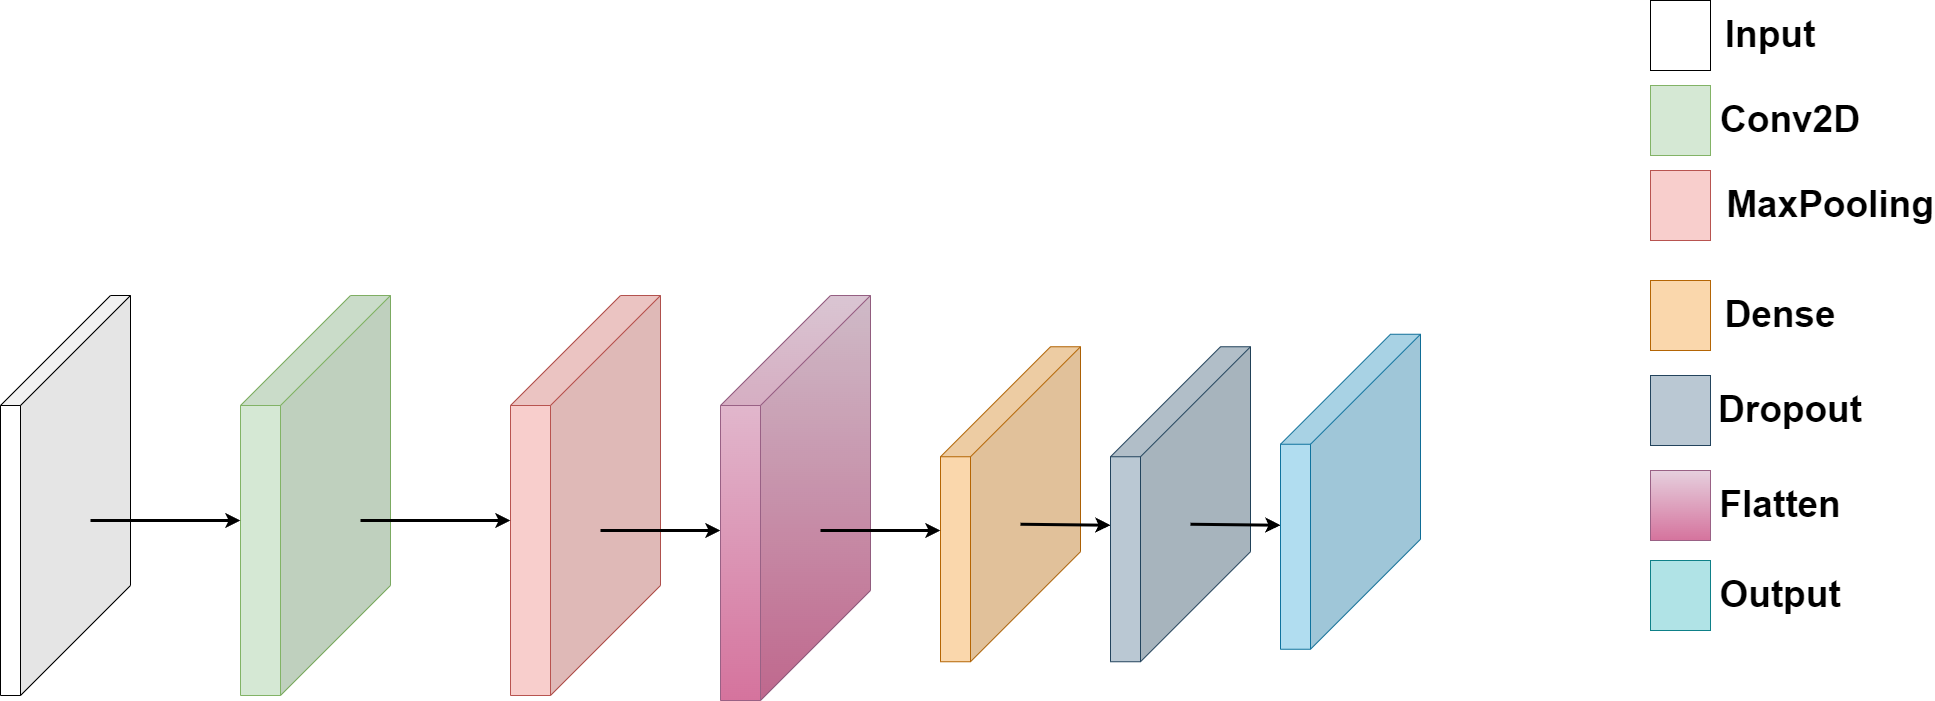
\includegraphics[width=0.8\linewidth]{gambar/bener/Arsitektur_CNN_Umum.png}
  % Keterangan gambar yang diinputkan
  \captionof{figure}{Arsitektur CNN}
  % Label referensi dari gambar yang diinputkan
  \label{fig:Arsitektur Umum Convolutional Neural Network}
\end{figure}
\textit{Convolutional Neural Network (CNN)} adalah sebuah jenis arsitektur model \textit{deep learning} yang khusus dirancang melaksanakan tugas-tugas pengolahan citra dan analisis visual. Inspirasi utama dari \textit{CNN} berasal dari cara otak manusia, khususnya korteks visual, memproses dan memahami informasi visual. Dengan menggunakan lapisan-lapisan konvolusi, \textit{CNN} dapat secara efektif dan efisien mengidentifikasi fitur-fitur penting dalam gambar secara hierarkis. Fungsi utama lapisan konvolusi dalam \textit{CNN} seperti pada \ref{fig:Arsitektur Umum Convolutional Neural Network}
adalah mendeteksi pola-pola spesifik atau fitur-fitur visual pada data input. Lapisan konvolusi dilengkapi dengan filter atau kernel kecil yang bergeser secara bertahap di seluruh citra agar menghasilkan peta fitur yang mencerminkan kehadiran fitur-fitur tersebut. Misalnya, filter pertama mungkin berfokus pada deteksi tepi dan garis, sementara filter berikutnya dapat mengenali sudut atau bentuk yang lebih kompleks. \cite{wu2017introduction}

Setelah melalui lapisan konvolusi, data diproses melalui lapisan aktivasi seperti \textit{ReLU (Rectified Linear Unit)}. Fungsi aktivasi ini membantu memperkenalkan non-linearitas ke dalam model, memungkinkan \textit{CNN} mempelajari representasi fitur yang lebih kompleks dan abstrak. Proses konvolusi dan aktivasi berulang pada lapisan-lapisan berikutnya, dengan setiap lapisan mencoba memahami dan mengekstraksi fitur-fitur semakin tingkat tinggi dari peta fitur sebelumnya. Selain lapisan konvolusi, \textit{CNN} juga mengandung lapisan-lapisan lain seperti \textit{pooling layer} dan \textit{fully connected layer}. \textit{Pooling layer} bertujuan mereduksi dimensi spasial dari peta fitur, mengurangi jumlah parameter dan mencegah overfitting. Kemudian, data hasil pooling diubah menjadi vektor dan diproses melalui \textit{fully connected layer} melakukan tugas klasifikasi atau regresi. \cite{koushik2016understanding}

Kekuatan utama dari \textit{CNN} adalah kemampuannya secara otomatis dan adaptif mempelajari representasi fitur dari data input. Dengan mendeteksi dan memahami fitur-fitur kunci dari gambar secara hierarkis, \textit{CNN} dapat menghasilkan prediksi atau output yang akurat dalam berbagai tugas analisis visual. Penggunaan teknologi \textit{deep learning} seperti \textit{CNN} telah menghadirkan perubahan signifikan dalam berbagai industri dan bidang, menciptakan solusi baru dan aplikasi yang inovatif dalam mengatasi masalah-masalah kompleks. Terus berlanjutnya penelitian dan pengembangan di bidang \textit{deep learning} diharapkan akan membuka lebih banyak potensi implementasi dan penerapan \textit{CNN} dalam berbagai konteks dan permasalahan dunia nyata. Contoh implementasi \textit{CNN} sangat beragam dan telah berhasil diterapkan dalam berbagai bidang. Misalnya, dalam klasifikasi gambar, \textit{CNN} telah digunakan ketika mengenali objek-objek pada gambar seperti manusia, mobil, atau binatang. Di bidang medis, \textit{CNN} dapat membantu dalam deteksi dan diagnosis penyakit berdasarkan gambar medis seperti X-ray atau MRI. Selain itu, dalam industri otomotif, \textit{CNN} digunakan dalam pengembangan kendaraan otonom agar bisa mendeteksi dan mengenali objek di sekitar kendaraan.

Implementasi dari \textit{Convolutional Neural Network (CNN)} telah menjadi salah satu pendorong utama dalam perkembangan teknologi dan aplikasi visual yang revolusioner. Dalam bidang komputer visi, \textit{CNN} telah digunakan dalam berbagai aplikasi seperti deteksi objek, segmentasi citra, dan rekonstruksi gambar. Penggunaan \textit{CNN} dalam industri otomotif juga semakin populer dalam pengembangan kendaraan otonom, di mana \textit{CNN} digunakan saat mendeteksi dan mengenali objek di sekitar kendaraan seperti pejalan kaki, kendaraan lain, dan rambu lalu lintas. Di bidang kesehatan, \textit{CNN} telah menemukan penerapan yang luas dalam analisis citra medis, termasuk deteksi kanker, segmentasi organ, dan pengenalan pola patologis. \textit{CNN} telah membantu mempercepat dan meningkatkan akurasi diagnosa medis, membuka peluang dalam penanganan penyakit secara lebih dini dan tepat.

Selain itu, aplikasi \textit{CNN} juga dapat ditemukan dalam industri hiburan dan kreatif. \textit{CNN} digunakan dalam teknologi realitas virtual dan \textit{augmented reality} ketika melacak gerakan pengguna dan mengintegrasikan objek virtual ke dalam lingkungan nyata. Dalam industri film dan animasi, \textit{CNN} memungkinkan penciptaan efek visual yang menakjubkan dan realistis. Penggunaan teknologi \textit{deep learning}, termasuk \textit{CNN}, telah memberikan dampak signifikan dalam bidang kecerdasan buatan dan telah menciptakan kemajuan besar dalam berbagai industri. Contoh arsitektur dari \textit{CNN} yang terkenal adalah \textit{LeNet-5}, yang dikembangkan oleh Yann LeCun pada tahun 1998 mengenali karakter tulisan tangan. Arsitektur \textit{LeNet-5} terdiri dari dua lapisan konvolusi yang diikuti oleh lapisan pooling dan lapisan terhubung penuh. \textit{LeNet-5} berhasil memperkenalkan konsep konvolusi dalam dunia pengolahan citra dan memberikan dasar bagi pengembangan model \textit{CNN} lebih lanjut.

Selanjutnya, ada arsitektur \textit{AlexNet} yang dikembangkan oleh Alex Krizhevsky, Ilya Sutskever, dan Geoffrey Hinton pada tahun 2012. \textit{AlexNet} merupakan salah satu arsitektur yang mempopulerkan penggunaan \textit{deep learning}, terutama \textit{CNN}, dalam tugas klasifikasi gambar. \textit{AlexNet} berhasil meraih kemenangan besar dalam kompetisi \textit{ImageNet} dengan performa yang jauh lebih baik dari metode konvensional pada saat itu. Selanjutnya, arsitektur \textit{VGGNet} dikembangkan oleh Karen Simonyan dan Andrew Zisserman pada tahun 2014. \textit{VGGNet} terkenal dengan kedalaman yang lebih besar, terdiri dari 16 atau 19 lapisan konvolusi, yang membantu meningkatkan akurasi dalam klasifikasi gambar dengan biaya komputasi yang lebih tinggi.

Contoh lainnya adalah arsitektur \textit{GoogLeNet} yaitu \textit{Inception} yang dikembangkan oleh tim dari \textit{Google} pada tahun 2014. \textit{GoogLeNet} memperkenalkan modul \textit{Inception} yang mencakup beberapa operasi konvolusi dalam paralel, mengoptimalkan kompromi antara akurasi dan efisiensi komputasi.Sejak saat itu, muncul berbagai arsitektur CNN lainnya, seperti \textit{ResNet}, \textit{DenseNet}, dan \textit{MobileNet}, yang terus mengalami pengembangan memenuhi kebutuhan beragam dalam berbagai aplikasi dan mendapatkan hasil yang lebih baik dalam analisis visual.

\subsubsection{ResNet50v2}
\textit{ResNet50V2} adalah salah satu model arsitektur \textit{Convolutional Neural Network (CNN)} yang merupakan variasi dari ResNet50, yang dikembangkan oleh Kaiming He dan timnya pada tahun 2015. ResNet sendiri merupakan singkatan dari \textit{Residual Network} yang merupakan terobosan dalam pengembangan jaringan saraf yang sangat dalam. Masalah utama yang diatasi oleh ResNet adalah pemudaran gradien yang sering terjadi pada jaringan yang dalam, yang menyebabkan kesulitan dalam pelatihan dan pengoptimalan model. \textit{ResNet50V2} menggunakan teknik \textit{Skip Connection} atau \textit{Residual Connections} mengatasi masalah pemudaran gradien ini. \cite{rahimzadeh2020modified} . Cara kerja \textit{ResNet50V2} seperti pada Gambar \ref{fig:ArsitekturResNet50V2}
dimulai dengan lapisan konvolusi pertama melakukan ekstraksi fitur dari gambar input. Setelah itu, model menggunakan beberapa blok residual bertingkat agar mempelajari representasi fitur yang semakin kompleks. Blok residual adalah inti dari arsitektur ResNet, yang memungkinkan aliran informasi yang lancar melalui lapisan-lapisan jaringan. \textit{Skip connections} memungkinkan input lompat langsung ke lapisan yang lebih dalam, atau ditambahkan ke output lapisan tersebut, sehingga memungkinkan model mempertahankan informasi asli selama proses pembelajaran.

\begin{figure}[!hbt]
  \centering
  % Nama dari file gambar yang diinputkan
  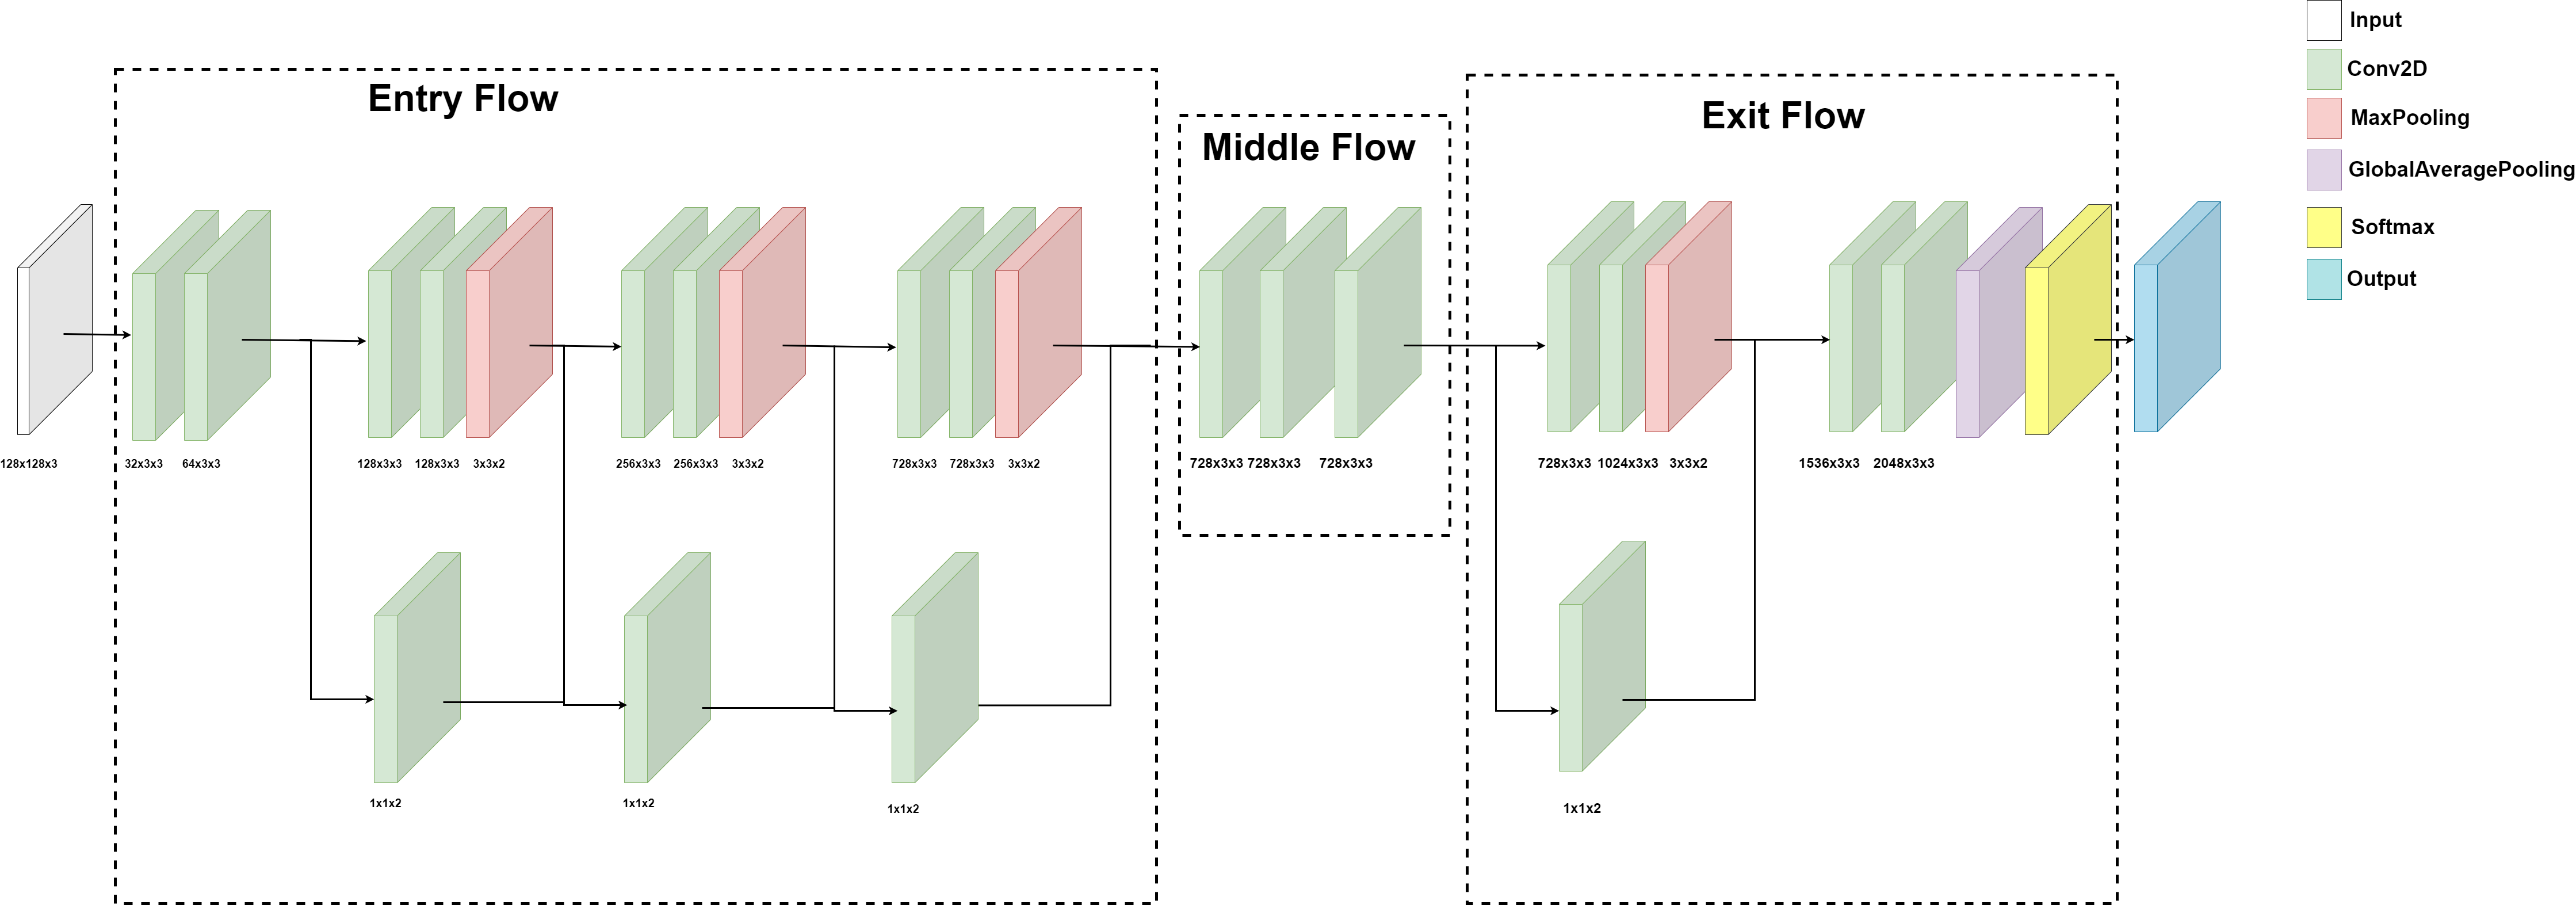
\includegraphics[width=0.8\linewidth]{gambar/bener/Arsitektur_ModelCNNResNet50V2_Dasar.png}
  % Keterangan gambar yang diinputkan
  \captionof{figure}{Arsitektur CNN ResNet50V2}
  % Label referensi dari gambar yang diinputkan
  \label{fig:ArsitekturResNet50V2}
\end{figure}

Dengan menggunakan blok residual dan \textit{skip connections}, \textit{ResNet50V2} dapat mengatasi masalah pemudaran gradien dengan lebih efektif. Gradien adalah indikator bagaimana model merespons perubahan parameter selama proses pelatihan. Pemudaran gradien terjadi ketika nilai gradien menjadi sangat kecil atau bahkan menghilang saat melewati lapisan-lapisan dalam jaringan. Dalam jaringan yang sangat dalam, pemudaran gradien dapat menyebabkan kesulitan dalam mengoptimalkan parameter dan memperlambat proses pelatihan. Namun, dengan adanya \textit{skip connections}, informasi dapat lebih mudah mengalir mundur melalui jaringan, mengurangi pemudaran gradien dan mempercepat pelatihan. \cite{prusty2022resnet50v2} . Selain itu, \textit{ResNet50V2} menggunakan blok \textit{"bottle-neck"} yang terdiri dari tiga lapisan konvolusi dengan ukuran kernel yang berbeda, yaitu 1x1, 3x3, dan 1x1. Penggunaan blok \textit{bottle-neck} ini mengurangi dimensi fitur di tengah blok, mengurangi kompleksitas komputasi dan jumlah parameter yang diperlukan. Dengan demikian, \textit{ResNet50V2} memiliki struktur yang lebih efisien dan dapat menghasilkan representasi fitur yang lebih kuat dengan meminimalkan biaya komputasi.

Selain teknik \textit{skip connections} dan blok \textit{bottle-neck}, \textit{ResNet50V2} juga menerapkan normalisasi batch (batch normalization) dan fungsi aktivasi \textit{ReLU} (Rectified Linear Unit) pada setiap lapisan konvolusi. Normalisasi batch membantu meningkatkan kestabilan dan kemampuan pembelajaran jaringan, sementara \textit{ReLU} berfungsi memperkenalkan non-linearitas dan meningkatkan representasi fitur yang dapat dipelajari oleh model. \textit{ResNet50V2} telah terbukti menjadi salah satu arsitektur yang sangat efektif dalam berbagai tugas pengolahan citra dan visi komputer. Model ini telah digunakan dalam banyak kompetisi dan tugas benchmark, menghasilkan performa yang luar biasa dalam klasifikasi gambar, deteksi objek, dan tugas-tugas visual lainnya. Dengan menggunakan kombinasi teknik canggih seperti skip connections, blok \textit{bottle-neck}, normalisasi batch, dan fungsi aktivasi \textit{ReLU}, \textit{ResNet50V2} berhasil mencapai tingkat akurasi yang tinggi dalam berbagai skenario dan aplikasi, menjadi salah satu pilihan utama terkait masalah pengolahan citra yang kompleks.

\subsubsection{Xception}
Arsitektur \textit{Xception} adalah inovasi dalam desain jaringan saraf tiruan yang menawarkan solusi efisiensi komputasi dan kinerja yang tinggi dalam tugas pengolahan citra. Cara kerja arsitektur \textit{Xception} berfokus pada penggunaan konsep konvolusi yang dapat dipisahkan secara mendalam agar mengurangi beban komputasi dan jumlah parameter dalam model. Ini menghasilkan model yang lebih ringkas dan cepat, sehingga lebih mudah dijalankan pada perangkat dengan sumber daya terbatas.

Konsep utama di balik \textit{Xception} adalah menggantikan operasi konvolusi standar dalam modul \textit{Inception} dengan konvolusi yang dapat dipisahkan secara mendalam seperti pada Gambar \ref{fig:ArsitekturXception}
. Modul \textit{Inception} adalah bagian kunci dari arsitektur jaringan \textit{Inception}, yang menggunakan berbagai ukuran \textit{filter} dalam paralel dalam mengekstraksi fitur dari gambar input. Dengan menggunakan konvolusi yang dapat dipisahkan secara mendalam, \textit{Xception} memisahkan operasi konvolusi menjadi dua tahap: konvolusi \textit{depthwise} dan konvolusi \textit{pointwise}.Pada tahap konvolusi \textit{depthwise}, satu \textit{filter} digunakan setiap lapisan input. Konvolusi ini dilakukan secara terpisah bagi setiap kanal warna (depth) gambar, yang menghasilkan output berukuran tinggi x lebar x kedalaman. Output dari langkah ini akan menjadi input dari tahap konvolusi \textit{pointwise}. Pada tahap konvolusi \textit{pointwise}, \textit{filter} dengan ukuran 1x1xkedalaman digunakan menghasilkan beberapa fitur. Penggunaan konvolusi 1x1 ini memungkinkan model melakukan operasi linier pada data input menghasilkan representasi fitur yang lebih kompleks.

\begin{figure}[!hbt]
  \centering
  % Nama dari file gambar yang diinputkan
  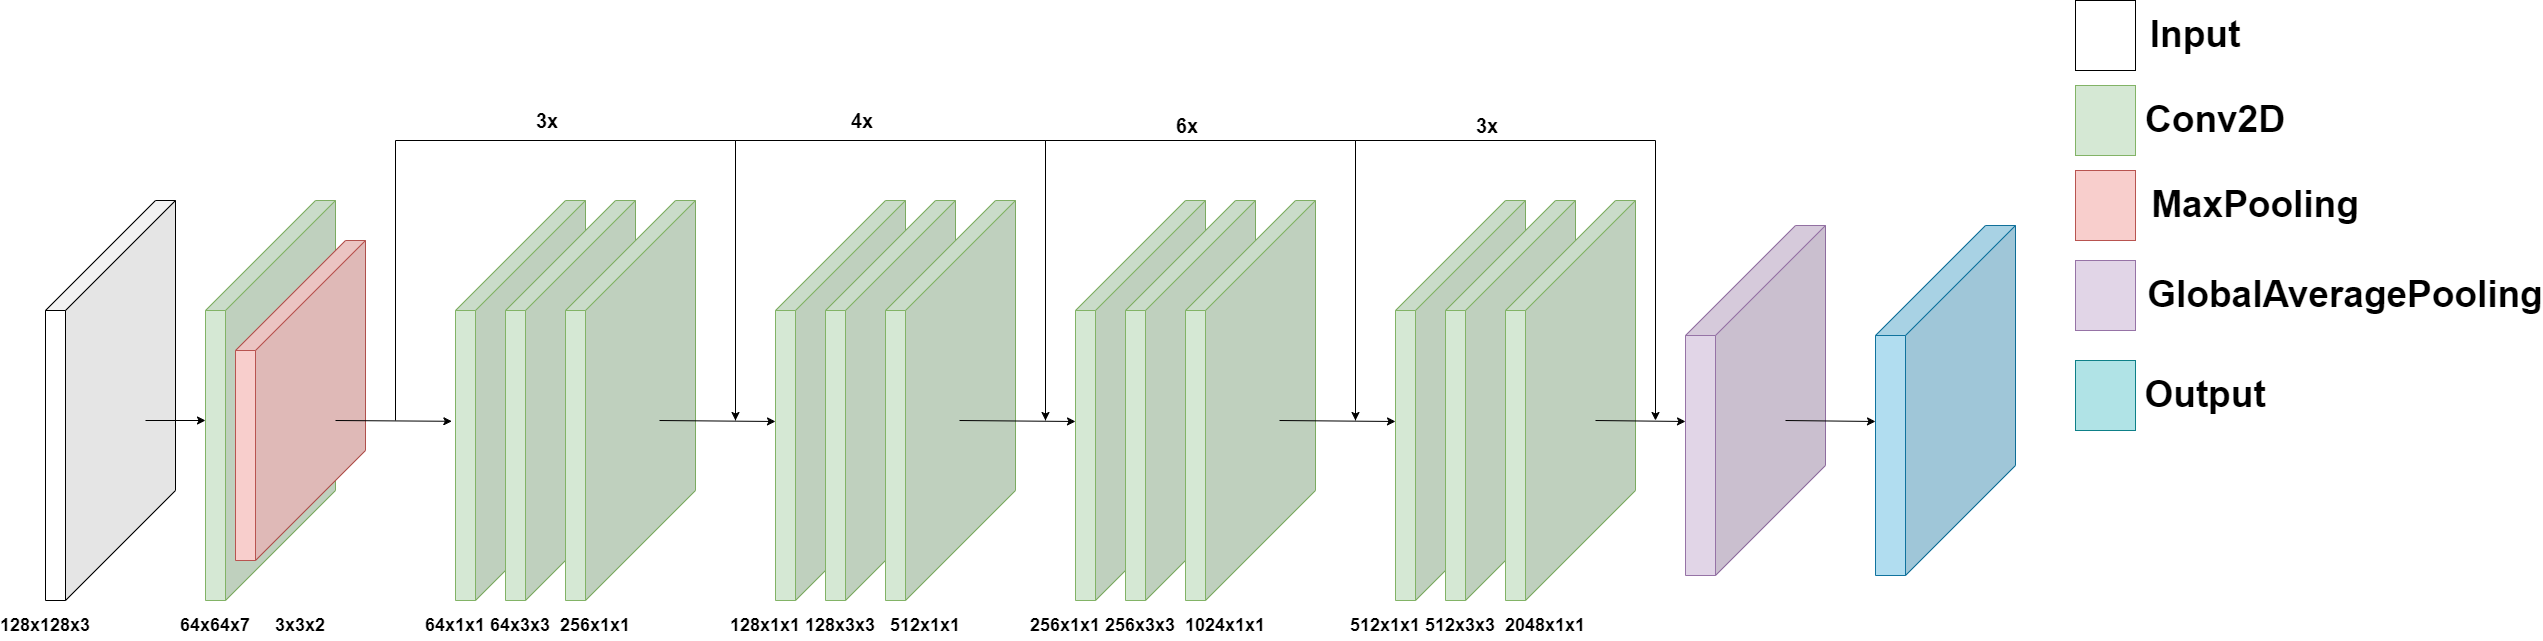
\includegraphics[width=0.8\linewidth]{gambar/bener/Arsitektur_CNNXception.png}
  % Keterangan gambar yang diinputkan
  \captionof{figure}{Arsitektur CNN Xception}
  % Label referensi dari gambar yang diinputkan
  \label{fig:ArsitekturXception}
\end{figure}
Struktur arsitektur \textit{Xception} terdiri dari tiga modul utama: \textit{entry flow}, \textit{middle flow}, dan \textit{exit flow}. \textit{Entry flow} terdiri dari konvolusi normal diikuti oleh konvolusi yang dapat dipisahkan secara mendalam. Modul ini bertanggung jawab menginisialisasi fitur-fitur penting dari gambar input. Selanjutnya, \textit{middle flow} terdiri dari 8 miniblock, setiap miniblock terdiri dari 3 konvolusi yang dapat dipisahkan secara mendalam. Modul ini bertanggung jawab melakukan proses ekstraksi fitur yang lebih mendalam dan kompleks dari gambar. Terakhir, \textit{exit flow} terdiri dari konvolusi yang dapat dipisahkan secara mendalam, feature flattening, dan output. Modul ini bertanggung jawab menghasilkan hasil akhir dari model, seperti prediksi kelas dalam tugas klasifikasi gambar.

Dengan menggunakan teknik konvolusi yang dapat dipisahkan secara mendalam, \textit{Xception} berhasil mengurangi jumlah parameter yang diperlukan dalam model dan meningkatkan efisiensi komputasi. Dalam model yang lebih dalam dan kompleks, jumlah perkalian matriks yang diperlukan melakukan konvolusi dapat sangat besar, menyebabkan model menjadi lebih lambat dan membutuhkan lebih banyak sumber daya komputasi. Dengan menggunakan konsep konvolusi yang dapat dipisahkan secara mendalam, \textit{Xception} mengurangi beban komputasi ini, sehingga model dapat dijalankan dengan lebih cepat dan lebih efisien.

Dalam berbagai tugas pengolahan citra, \textit{Xception} telah terbukti memberikan hasil yang sangat baik dan akurasi yang tinggi. Model ini telah digunakan dalam berbagai kompetisi dan benchmark, menunjukkan kinerja yang unggul dalam klasifikasi gambar, deteksi objek, segmentasi citra, dan tugas visual lainnya. Kemampuan \textit{Xception} menghasilkan representasi fitur yang kuat dan kompresi model yang efisien menjadikannya pilihan utama dalam berbagai aplikasi pengolahan citra dan visi komputer. Dengan terus berkembangnya teknologi deep learning, \textit{Xception} terus menjadi subjek penelitian dan pengembangan meningkatkan performa dan kemampuannya dalam berbagai tugas pengolahan citra yang semakin kompleks dan realistis.



